\documentclass{beamer}

\usepackage[utf8]{inputenc}
\usepackage[T1]{fontenc}
\usepackage{lmodern}
\usepackage{microtype}

\usepackage{color}
\usepackage{tikz}

\usepackage{amssymb}
\usepackage{amsmath}

\addtobeamertemplate{navigation symbols}{}{%
    \usebeamerfont{footline}%
    \usebeamercolor[fg]{footline}%
    \hspace{1em}%
    \insertframenumber
}


\begin{document}
\title{Strengthening memory safety in Rust:\\
Exploring CHERI capabilities for a safe language}
\author{Nicholas Sim}
\date{June 21, 2019}

\frame{\titlepage}


\begin{frame}
\frametitle{Why memory safety is important}

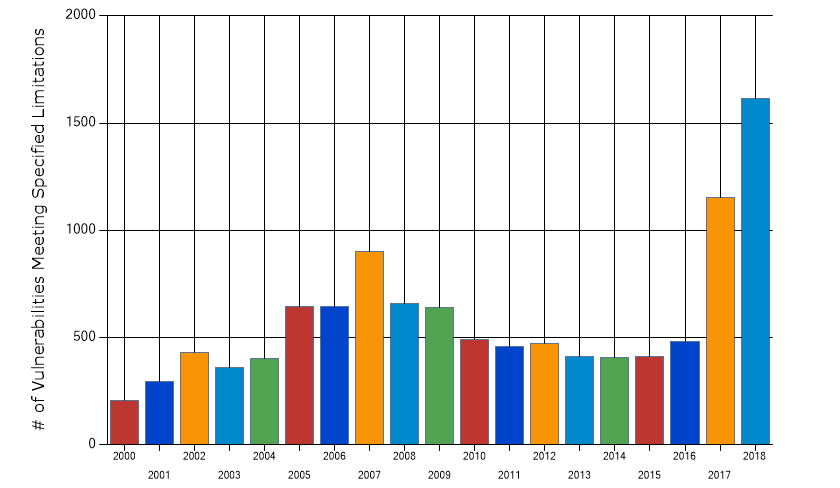
\includegraphics[width=\textwidth]{graph-overflow.png}
\begin{itemize}
    \item Buffer overflows \emph{still} on the rise [fig.: NIST NVD]
\end{itemize}
\end{frame}


\begin{frame}
\frametitle{CHERI: capablity architecture}

\begin{itemize}
    \item An instruction set architecture, extends RISC
    \item Offers hardware capabilities: unforgeable tokens for pointers
    \item Protects memory from unauthorised access
    \item MORE
    \item Under development here
    \item Mainly studied under C: capabilities known to be effective for
    unsafe languages
\end{itemize}
\end{frame}

\begin{frame}
\frametitle{Rust: safe language}

\begin{itemize}
    \item New programming language (c.\ 2012)
    \item Rust's models ``guarantee memory safety'' (big claim!)
    \item Boasts of performance \emph{and} memory safety
    \item Recognises that C is too complex, too much undefined behaviour\footnote{viz.\ Memarian et al.\ 2016}
    \item Split into \emph{Safe}, \emph{Unsafe} Rust
    \item For safety and power respectively
    \item (New slide here?)
    \item 7 vulnerabilities and counting in standard library + compiler
    \item 5 of these fully prevented by capabilities!
\end{itemize}
\end{frame}

\end{document}